
\subsection{Пример 1: Выбор наиболее привлекательных инновационных технологий}

Этот пример построен вокруг реального проекта, где наша методика проведения экспертного опроса использовалась крупным российским инвестором. %для оценки инвестиционной привлекательности инновационных  технологий.

Имеется множество инновационных технологий $O$ размера $\abs{O} = N$.  Технология --- результат научно-технической деятельности, который включает в себя изобретения, промышленные образцы, компьютерные программы, технические данные или другие результаты интеллектуальной деятельности и может служить основой определённой практической, в том числе коммерческой деятельности. Каждая технология имеет одного или нескольких правообладателей, получающих выгоду от её применения в практической деятельности. Технологии являются инновационными в том смысле, что обладают значительной новизной и гипотетически имеют большой потенциал для развития, внедрения и получения прибыли, но всё это сопровождается значительным риском. 

%Если делать акцент не на самой технологии, а на команде людей, которые заняты разработкой и практическим применением технологии, то говорят об инновационном проекте или инновацонной компании. Всё, что ниже сказано про оценку технологий, остаётся верно и для оценки компаний с точностью до выбора критериев оценки.
%Есть крупный инвестор, у которого есть возможность стать совладельцем или полным владельцем технологии, если он вложит деньги и иные ресурсы в её развитие, вступив в сделку с текущими правообладателями. 
% (и так очевидно)

С точки зрения инвестора, технологии обладают разной инвестиционной привлекательностью, которая оценивается исходя из нескольких аспектов технологии, среди которых: доходность технологии через год после приобретения, её востребованность на рынке, конкурентоспособность, затраты на внедрение, потенциал интеллектуальной собственности, потенциал кадрового обеспечения, экологические риски, административные риски и т.\,д. 

Пусть привлекательность технологии по всем важным аспектам выражается числами $x_1 \in X_1, x_2 \in X_2, ...$, где мы для простоты положили $X_1 = X_2 = ... = \{0, ..., 10\}$. Инвестиционная привлекательность получается из этих чисел с помощью обычных операций сложения, перемножения и умножения на некоторые коэффициенты в соответствии со специально разработанной блок-схемой (рис.~\ref{ris:tech_scheme}), которая графически выражает функцию $f: x = f(x_1, x_2, ...)$. 

Были приглашены несколько экспертов. Каждого эксперта мы попросили оценить каждую технологию по каждому аспекту. Использовались нечёткие оценки, представленные в виде таблицы <<балл (значение $x \in \{0, ..., 10\}$) --- оценка (значение $p_{\tilde x}(x)$)>>, см.~рис.~\ref{ris:expert_sample}. В нашем случае выделялось $M = 16$ крупных аспектов с отдельными оценками. При этом с точки зрения методологии каждый из этих аспектов <<вобрал в себя>> ряд более мелких подпунктов примерно одинаковой важности, которые уже не требовали отдельных оценок во избежание чрезмерной нагрузки на эксперта. В документе-описании, который выдавался каждому эксперту, все аспекты расшифрованы: указано, какие подпункты мы рассматриваем и о чём следует  подумать перед выставлением оценки по каждому аспекту.

\begin{figure}[H]
\center{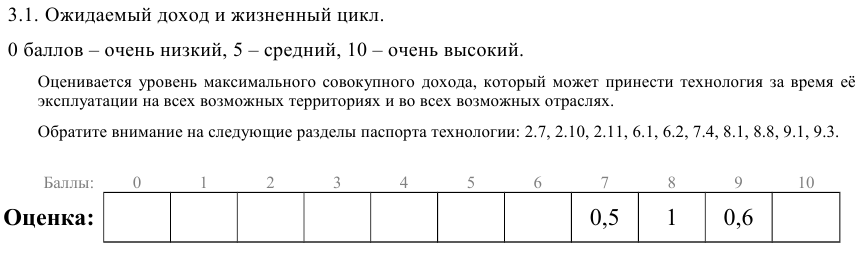
\includegraphics[width=0.85\linewidth]{./pic/expert_sample}}  % this is temporarily changed!!!
\caption{\small Блок-схема, иллюстрирующая конкретный вид функции $f: x = f(x_1, x_2, ...)$, объединяющей различные аспекты инновационной технологии, оцениваемые экспертом, в итоговую величину инвестиционной привлекательности технологии. }
\label{ris:tech_scheme}
\end{figure}

 
\begin{figure}[H]
\center{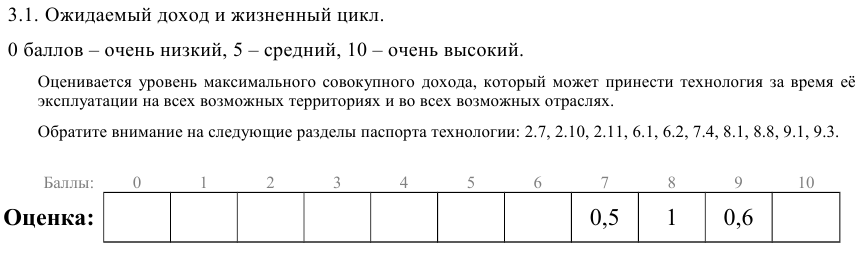
\includegraphics[width=0.85\linewidth]{./pic/expert_sample}}
\caption{\small Пример заполненного фрагмента листа экспертного опроса, проведённого по нашей методике. Эксперт выставил нечёткую оценку в ячейках таблицы <<балл (значение $x$) --- оценка (значение $p_{\tilde x}(x)$)>>. Пустым клеткам таблицы соответствуют значения $p_{\tilde x} = 0$. }
\label{ris:expert_sample}
\end{figure}

Интересно отметить, что для различных рисков и других негативных аспектов технологии большие числовые значения в таблице интуитивно соответствуют более плохой ситуации, более низкому <<качеству>> объекта. Но поскольку $f$ должна быть монотонна по всем аргументам, требуется единообразие, например, увеличение аргументов $f$  всегда приводит к более высокому значению $f$, т.\,е. более высокому <<качеству>>. Поэтому мы сделали дополнительные указания для экспертов в тех местах, где большие числовые значения интерпретируются как более низкий риск. Этого можно избежать, если делать предварительную обработку оценок: автоматически отразить оценки, нарушающие монотонность, вдоль оси абсцисс (баллов) вокруг оси, проходящей через середину диапазона баллов.

Совокупность сырых экспертных оценок была загружена в программу расчёта коллективной оценки. Полученное коллективное мнение было загружено в программу, реализующую быстрый алгоритм нахождения возможности не попасть в $k$ лидеров для каждой из технологий, которых в нашем случае набралось $N = 15$ штук. Мы запускали программу при разных значениях $k = 1, 2, 3, 4, 5$. Вывод программы был представлен в виде столбика значений $\P_l, l \in \setN$, поскольку эту информацию нельзя сократить без потерь (см. Замечания в разделе Задача оптимального выбора группы объектов.)
% результат оправдал ожидания
%TODO: нужны графики ?

\subsection{Пример 2: Выбор оптимальных реактивов для маркировки белков в цикле ***}

Этот пример посвящён важной области применения экспертных опросов на стыке естественных наук и экономики --- области планирования эксперимента. 

Одним из центральных вопросов для науки биохимии является вопрос о том, какие химические реакции протекают в живом организме, и какие вещества участвуют в этих реакциях. Как правило, исследуют т.\,н. циклы реакций с участием белков. В живом организме встречается много тысяч различных белков и добрая сотня из них участвует в исследуемом цикле реакций. Концентрация веществ, участвующих в реакциях, в частности -- белков, как правило, изменяется на отдельных стадиях цикла реакций, и может изменяться в результате полного цикла.

Для идентификации конкретного белка и определения его концентрации служат специальные реактивы, причём один реактив может обладать активностью сразу к нескольким белкам (и заранее неизвестно, к каким?). Биологи контролируют изменение концентрации выбранных белков в некоторой точке организма таким образом, что организм не погибает (и вмешательство в его работу минимально?) По каждому белку есть предположения относительно того, насколько возможно, что: (1) его количество уменьшится, (2) не изменится, (3) увеличится. В силу некоторых причин, в том числе, но не ограничиваясь дороговизной реактивов, мы можем контролировать только небольшое количество белков, как правило, в пределах $10$.

Объекты -- белки. <<Качество>> белка складывается из того, какие белки, по мнению эксперта, участвуют в цикле (и их имеет смысл контролировать), и насколько дорогой реактив требуется для контроля. Эксперт оценивает для каждого белка $i \in \setN$ возможность $\p_{ij}(x)$ обнаружения изменения его концентрации на $x$ процентов (или чего там, логарифма какого-нибудь) с помощью реактива $j \in \setM$. Цены различных реактивов учтены в $f(\cdot)$ как коэффициенты перед $x_{ij}$ для разных $j$.

%Объекты -- реактивы. <<Качество>> реактивов складывается из того, какие белки, по мнению эксперта, участвуют в цикле. Эксперт оценивает для каждого реактива $i \in \setN$ возможность $\p_{ij} обнаружения каждого белка $j \in \setM$ (довольно много оценок, трудно для эксперта?). Нечёткий вектор $\theta: \p_{\theta} = \inf \p_{ij}$ не имеет смысла, т.\,к. (а) я забыл про баллы, ещё одно измерение и (б) при таком выборе нет независимости компонент, потому что есть априорные возможности обнаружить белок в реакции идеальным реактивом.    

%Выбор измерительного прибора мы будем рассматривать в контексте теории измерительно-вычислительнх преобразователей как средств измерений (ИВП) Ю.~П.~Пытьева \cite{4}. 


